%! Author = alireza
%! Date = 8/15/20

% Preamble
\documentclass[a4paper,12pt]{article}


% Packages
\usepackage{amsmath}
\usepackage{graphicx}
\usepackage{amsthm}
\newtheorem{thm}{Theorem}
\newtheorem*{numlessthm}{Theorem}
\usepackage{color}
\usepackage{hyperref}
\hypersetup{
    colorlinks=true,
    linkcolor=black,
    urlcolor=red,
    linktoc=all
}

% Document
\begin{document}

    \title{Linear algebra}
    \author{Alireza Qanbari}
    \date{\today}

    \maketitle


    \tableofcontents
    \newpage


    \section{Vector spaces}



    Until the 19th century, linear algebra was introduced through systems
    of linear equations and matrices. In modern mathematics, the presentation
    through
    vector spaces is generally preferred, sin
    ce it is more synthetic, more general (not limited to the finite-dimensional case),
    and conceptually simpler, although more abstract.

    A vector space over a field F (often the field of the real numbers) is a set V equipped with
    two binary operations satisfying the following axioms. Elements of V are called vectors, and elements of F are
    called scalars. The first operation, vector addition, takes any two vectors v and w and outputs a third vector
    v + w. The second operation, scalar multiplication, takes any scalar a and any vector v and outputs a new vector
    av. The axioms that addition and scalar multiplication must satisfy are the following. (In the list below, u, v
    and w are arbitrary elements of V, and a and b are arbitrary scalars in the field $F$.)\cite{2}


    \begin{center}


        \begin{tabular}{||l || l||}
            \hline
            Axiom & Signification \\
            \hline
            Associativity of addition &  $u+(v+w)=(u+v)+w$  \\
            \hline
            Commutativity of addition & $u+v=v+u$ \\
            \hline
            Identity element of addition & There exists an element 0 in V,\\
            &called the zero vector (or simply zero),\\
            & such that v + 0 = v for all v in V. \\
            \hline


        \end{tabular}
    \end{center}

    The first four axioms mean that V is an abelian group under addition.

    An element of a specific vector space may have various nature; for example, it could be a sequence, a function,
    a polynomial or a matrix. Linear algebra is concerned with those properties of such objects that are common to
    all vector spaces.


    \begin{figure}[h]
        \begin{center}


            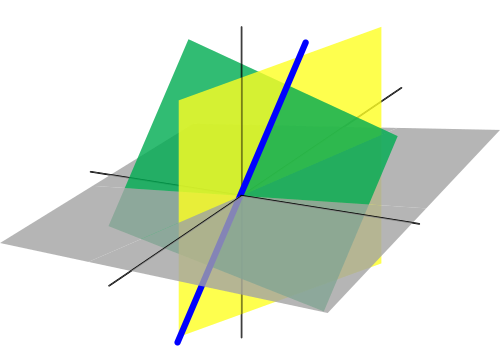
\includegraphics[width=0.3\textwidth]{pic1.png}
            \caption{
                \scriptsize {
                    In three-dimensional Euclidean space, these three planes represent solutions of linear equations,
                    and their intersection represents the set of common solutions: in this case, a unique point. The blue line is
                    the common solution to two of these equations.
                }
            }
        \end{center}

    \end{figure}

    \subsection{Linear maps}
    \label{maps}
    \textbf{Linear maps} are mappings between vector spaces that preserve the vector-space structure. Given two vector
    spaces V and W over a field F, a linear map (also called, in some contexts, linear transformation or linear mapping)
    is a map

    $$T:V\to W$$

    that is compatible with addition and scalar multiplication, that is
    $$T(u+v)=T(u)+T(v),\quad T(av)=aT(v)$$
    for any vectors u,v in V and scalar a in F.

    This implies that for any vectors u, v in V and scalars a, b in F, one has
    $$T(au+bv)=T(au)+T(bv)=aT(u)+bT(v)$$

    When $V = W$ are the same vector space, a linear map $T:V\to V$ is also known as a linear operator on $V$.

    A bijective linear map between two vector spaces (that is, every vector from the second space is associated with
    exactly one in the first) is an isomorphism. Because an isomorphism preserves linear structure, two isomorphic
    vector spaces are "essentially the same" from the linear algebra point of view, in the sense that they cannot be
    distinguished by using vector space properties. An essential question in linear algebra is testing whether a linear
    map is an isomorphism or not, and, if it is not an isomorphism, finding its range (or image) and the set of elements
    that are mapped to the zero vector, called the kernel of the map. All these questions can be solved by using
    Gaussian elimination or some variant of this algorithm.

    \subsection{Subspaces, span, and basis}
    \label{span}
    The study of those subsets of vector spaces that are in themselves vector spaces under the induced operations is
    fundamental, similarly as for many mathematical structures. These subsets are called linear subspaces. More
    precisely, a linear subspace of a vector space $V$ over a field $F$ is a subset $W$ of $V$ such that $u+v$ and au are
    in $W$, for every $u, v$ in W, and every $a$ in $F$. (These conditions suffice for implying that $W$ is a vector space.)


    For example, given a linear map $T:V\to W$ , the image $T(V)$ of $V$, and the inverse image $ T^{-1}(0)$
    of 0 (called kernel or null space), are linear subspaces of $W$ and $V$, respectively.
    Another important way of forming a subspace is to consider linear combinations of a set S of vectors: the set of
    all sums
    $$ a_{1}v_{1}+a_{2}v_{2}+\cdots +a_{k}v_{k}, $$

    where $v_{1}+v_{2}+\cdots +v_{k}$ are in $S$, and $a_{1}+a_{2}+\cdots +a_{k}$, ak are in $F$ form a linear subspace
    called the span of $S$. The span of S is also the
    intersection of all linear subspaces containing $S$. In other words, it is the (smallest for the inclusion relation)
    linear subspace containing $S$.

    A set of vectors is linearly independent if none is in the span of the others. Equivalently, a set $S$ of vector is
    linearly independent if the only way to express the zero vector as a linear combination of elements of $S$ is to
    take zero for every coefficient

    A set of vectors is linearly independent if none is in the span of the others. Equivalently, a set $S$ of
    vector is linearly independent if the only way to express the zero vector as a linear combination of elements
    of $S$ is to take zero for every coefficient $a_{i}$

    A set of vectors that spans a vector space is called a spanning set or generating set. If a spanning set $S$ is
    linearly dependent (that is not linearly independent), then some element $w$ of $S$ is in the span of
    the other elements of $S$, and the span would remain the same if one remove $w$ from $S$. One may continue
    to remove elements of $S$ until getting a linearly independent spanning set. Such a linearly independent set
    that spans a vector space $V$ is called a basis of $V$. The importance of bases lies in the fact that there are
    together minimal generating sets and maximal independent sets. More precisely, if $S$ is a linearly independent set,
    and $T$ is a spanning set such that $S\subseteq T,$ then there is a basis B such that $S\subseteq B\subseteq T.$

    Any two bases of a vector space $V$ have the same cardinality, which is called the dimension of $V$; this
    is the dimension theorem for vector spaces. Moreover, two vector spaces over the same field $F$ are isomorphic
    if and only if they have the same dimensio.\cite{3}

    If any basis of $V$ (and therefore every basis) has a finite number of elements, $V$ is a finite-dimensional vector
    space. If $U$ is a subspace of $V$, then $dim U \leq dim V$. In the case where $V$ is finite-dimensional, the equality of
    the dimensions implies $U=V$.


    If $U_1$ and $U_2$ are subspaces of $V$, then

    $$\dim(U_{1}+U_{2})=\dim U_{1}+\dim U_{2}-\dim(U_{1}\cap U_{2}),$$

    where $U_{1}+U_{2}$ denotes the span of $ U_{1}\cup U_{2}.$\cite{4}


    \newpage



    \begin{thebibliography}{ 9}

        \bibitem{1} {
            Benjamin Peirce (1872) Linear Associative Algebra, lithograph, new edition with corrections, notes,
            and an added 1875 paper by Peirce, plus notes by his son Charles Sanders Peirce, published in
            the American Journal of Mathematics v. 4, 1881, Johns Hopkins University, pp. 221 226, Google Eprint}
        \bibitem{2} {
            and as an extract, D. Van Nostrand, 1882, Google Eprint.}
        \bibitem{3} {
            Roman (2005, ch. 1, p. 27)}
        \bibitem{4} {
            Axler (2004, p. 55)}
    \end{thebibliography}
    \addcontentsline{toc}{section}{References}


\end{document}